\documentclass{SCreport}
\usepackage[utf8]{inputenc}
\usepackage[T1]{fontenc}
\usepackage{caption}
\captionsetup{labelsep=period}
\usepackage{float}
\usepackage[bottom]{footmisc}\renewcommand\footnotelayout{\,}
\usepackage{hyperref}
\captionsetup{font=small}
% GitHub commands
\newcommand\blob
{https://github.com/PacificCommunity/ofp-sam-transition-plan/blob/main}
\newcommand\ofpsam{https://github.com/PacificCommunity/ofp-sam}
\newcommand\present{\blob/presentations}
\newcommand\tree
{https://github.com/PacificCommunity/ofp-sam-transition-plan/tree/main}
% GitHub commands
\newcommand\cpp{\mbox{C\raisebox{0.5ex}{\tiny\bfseries ++}}}
\newcommand\h[1]{\hspace{#1}}
\newcommand\I[1]{\rule{0pt}{#1}}
\reporttype{SC21}
\reportauthor{A.~Magnusson\footnote{\spc}, N.~Davies\footnote{TeTakina Ltd},
  G.~Pilling$^1$, P.~Hamer$^1$}
\reporttitle{Scoping the Next Generation of Tuna Stock Assessment
  Software:\\Progress Report (Project 123)}
\reportnumber{\tpnum/SA-WP-01}
\reportdate{28 July 2025}
\setlength\hyphenpenalty{2000}
\setlength\tolerance{2000}
\hyphenation{implementing}
\begin{document}

\wcpfctitlepage

\tableofcontents
\newpage

\section{Executive summary}

\vspace{-1ex}

The 3-year Project 123 aims to examine and evaluate options for transitioning
WCPFC stock assessments from MULTIFAN-CL to other software. At SC20, ISG-09
reviewed the scoping of next-generation tuna stock assessment software and
supported prioritizing practical tasks, including transitioning swordfish and
striped marlin assessments to Stock Synthesis and testing simplified models for
yellowfin tuna. Members acknowledged the need to focus on immediate assessment
priorities while keeping longer-term software development under consideration,
depending on available resources and capacity. (SC20 Summary Report, Attachment
E).

SC21 will review the progress of Project 123, and this report presents progress
against each of the project TORs. Some of the WCPFC tuna stocks have specific
requirements for future assessments. For example, skipjack should use the
state-of-the-art statistical techniques for analyzing tagging data, while
albacore may transition to software that can incorporate close-kin
mark-recapture data that are currently being collected. A new statistical
approach that looks promising for analyzing skipjack tagging data uses an
external DTU spatio-temporal model. This method produces abundance indices that
can be incorporated into any stock assessment platform, such as Stock Synthesis.

One outcome from reaching out to tuna RFMOs is that IATTC has outlined a general
design for developing a new tuna model based on RTMB. This development work
stream will be initiated with an online CAPAM workshop on this topic. Compared
to an IATTC designed model in RTMB, the FIMS pathway to developing a new tuna
stock assessment software is subject to somewhat higher levels of uncertainty
and risks. Nevertheless, Project 123 is planning an SPC-FIMS workshop to examine
and evaluate the FIMS development option. The Gadget software represents key
statistical methods of interest, and the scoping project will examine this model
as a useful reference for designing any future tuna assessment software.
Ultimately, there are important benefits in using the same software as other
tuna RFMOs. The WCPFC partnership with IATTC is especially relevant for
collaborative research and development of new stock assessment software.

SC21 will provide feedback on the progress of the project as needed.

We invite SC21 to:\\[-4ex]

\begin{itemize}
  \item note that the scoping project is establishing partnerships with IATTC
  and the Technical University of Denmark (DTU) focusing on developing new
  software;\\[-4.5ex]
  \item note that in 2025, the two billfish stock assessments, swordfish and
  striped marlin, transitioned from MULTIFAN-CL to Stock Synthesis;\\[-4.5ex]
  \item review and comment on three possible software development work streams,
  described in this report (\autoref{sec:tor-7}), providing feedback that will
  guide the preparation of project proposal to be presented to SC22;
  and\\[-4.5ex]
  \item convene an ISWG to discuss the progress and develop activities and a TOR
  for the third year of Project 123.
\end{itemize}

\section{Background}

Following the retirement of the lead developer of MULTIFAN-CL (MFCL), Dave
Fournier, future advances to the MFCL software are not expected to be as
mathematically innovative as they were in the past. While this does not render
MFCL obsolete in the medium-term, it flags the need to plan and identify whether
alternative existing software exists, or new software must be developed in the
longer-term, to continue to support the specificities and future requirements of
WCPFC tuna stock assessments.

While MFCL (Fournier et al. 1998) continues to be improved to service the WCPFC
tuna assessment needs over at least the next 5+ years, it is important to start
on a phased approach to its replacement. An initial scoping phase is required to
assess what features and capabilities will be important in future assessment
software for tunas. This scoping phase will benefit from input from stock
assessment scientists across global tuna RFMOs. Once this scoping phase is
conducted, consideration of available software packages in relation to the
desired features and capabilities can be conducted. This may identify suitable
existing software that has potential to provide the desired features and/or has
potential to be developed further. Alternatively, it may indicate whether
embarking on development of a new software package is recommended.

There has also been discussion around the need to explore, through
modeling/simulation exercises, the benefits of applying alternative assessment
structures (i.e., length-age structured versus the traditional length-based
age-structured approach of MFCL and Stock Synthesis) before embarking on major
software developments or changing methodology. Similar can be said about
exploring benefits of state-space models and their use of random variables.
Recent developments in external tagging data analysis also opens up
possibilities to utilize SPCs tagging data with other software, and the
application of close-kin mark-recapture (CKMR) needs be an important part of our
considerations, given the work in this area on South Pacific albacore.

An important outcome of this work would be to ultimately have a software package
that has the desired functionality for tuna assessments, not only for WCPFC but
also for other tuna RFMOs, thus creating a user community and ongoing
development support capacity, so as to avoid the current situation we are facing
with MFCL. Wider collaboration in this venture is essential to achieving this
and is expected to be encouraged through this project.

The project website (\href{\ofpsam-transition-plan}{\ofpsam-transition-plan})
contains the main documents, presentations, workshops, and notes related to the
project.

\vspace{2ex}

\subsection{TOR summary}

The project terms of reference established at SC20 are listed in
\autoref{tab:tors}.

\newpage

\begin{table}
  \renewcommand\arraystretch{1.25}
  \centering
  \captionsetup{width=0.90\textwidth}
  \caption{Terms of reference established at SC20, guiding the project
    activities conducted from August 2024 to August 2025.\label{tab:tors}}
  \vspace{1ex}
  \begin{tabular}{p{1cm}p{13cm}}
    \hline
    TOR & Description\\
    \hline
    \hyperlink{link:tor-1}{1}
        & Review and identify a list of necessary features for software to do
          tuna stock assessments and identify existing software platforms that
          have these features or capacity to develop these.\\
    \hline
    \hyperlink{link:tor-2}{2}
        & Conduct two workshops with selected experts from other tuna RFMOs
          and/or with relevant expertise. The first workshop can be remote
          (prior to SC20) and the second one potentially in person (post SC20).
          The main goal will be to communicate the scoping project, upcoming
          model explorations, and succession plans for MFCL and Stock Synthesis,
          to seek advice from the scientific community, and to seek
          collaboration with tRFMOs and various research labs.\\
    \hline
    \hyperlink{link:tor-3}{3}
        & Explore the new RTMB programming environment and how it could be used
          in future tuna assessments. Specifically, how to modularize and
          organize code in RTMB models, on one hand code that is specific to one
          assessment and on the other hand code that is shared between
          assessments.\\
    \hline
    \hyperlink{link:tor-4}{4}
        & Establish collaboration with NOAA scientists to explore the
          feasibility of enhancing the tagging module in Stock Synthesis, making
          it more similar to the tagging module in MFCL.\\
    \hline
    \hyperlink{link:tor-5}{5}
        & Provide support to the stock assessment team transitioning the 2025
          swordfish assessment from MFCL to Stock Synthesis. Also, coordinate
          with the 2024/2025 striped marlin assessment team to start preparing
          for the transition of that assessment to Stock Synthesis in 2029.\\
    \hline
    \hyperlink{link:tor-6}{6}
        & Compare a variety of software platforms using a simplified
          single-region WCPO yellowfin tuna dataset. The comparison will
          evaluate available features, run time speed, auxiliary tools, time and
          skills required to develop and diagnose models, and other
          characteristics.\\
    \hline
    \hyperlink{link:tor-7}{7}
        & Prepare alternative workplans and budget scenarios for the larger
          implementing (main) project to go beyond scoping. The scoping project
          will be expected to transition into the main implementing project
          based on the discussions at SC21, budget considerations, and funding
          availability. It is expected that the work leading up SC21 will inform
          the implementing workplan options and budget estimations.\\
    \hline
    \hyperlink{link:tor-8}{8}
        & Communicate with tuna RFMOs and other research labs to establish which
          RFMOs and labs are willing and able to commit scientist time to
          collaborate on specific tasks of the scoping project, as well as the
          upcoming main project.\\
    \hline
    \hyperlink{link:tor-9}{9}
        & Communicate with tuna RFMOs and the FIMS project team to evaluate
          whether joint software development by tuna RFMOs could produce FIMS
          code modules, with the aim to develop future tuna assessment models
          using FIMS modules.\\
    \hline
  \end{tabular}
\end{table}

\clearpage

\section{Progress against TOR items}

This section describes the project activities in the last 12 months from August
2024 to August 2025, as they relate to terms of reference 1--9 that were
established at SC20.

\vspace{1ex}

\hypertarget{link:tor-1}{}
\subsection{TOR work area 1 (2024 second half)}
\label{sec:tor-1}

\begin{quote}\sf
  Review and identify a list of necessary features for software to do tuna stock
  assessments and identify existing software platforms that have these features
  or capacity to develop these.
\end{quote}

\vspace{2ex}

A question was raised at SC20 about whether it would be possible to present a
review and evaluation of necessary software features and existing software. This
is provided below in one section covering software features and another section
covering existing software.

\subsubsection{Evaluation of necessary software features}

\vspace{1ex}

\textbf{Software features listed at CAPAM 2019 workshop}

\vspace{1ex}

The CAPAM 2019 Workshop on Next Generation Assessment Models produced a review
paper (Punt et al. 2020) that identifies a number of model features considered
important in future stock assessment software. The abstract of the review paper
lists these features:

\begin{itemize}
  \item Ability to to capture age and size dynamics simultaneously yet
  computationally efficiently, while also offering the option to run a model as
  purely age-structured for a simple and fast model
  \item Scale from data-rich to data-poor
  \item Include some multispecies capability
  \item More appropriately deal with temporal variation, e.g., random effects
  and state-space models
  \item Better handling of tagging data, e.g., release-conditioned or
  recapture-conditioned model
  \item Ability to use close-kin mark-recapture data
  \item Efficient methods to share parameter priors among stocks, borrowing
  information from similar stocks where more data have been collected
  \item Training programs and documentation
  \item Data entry system that is well documented
  \item Does not require specification of inputs that will not be used in an
  application
  \item Expert system to configure default settings based on best practices
  \item Automatic production of diagnostic statistics
\end{itemize}

\vspace{2ex}

The summary table in Punt et al. (2020) adds the following features:

\begin{itemize}
  \item Spatial structure
  \item Multiple fisheries and surveys
  \item Flexible parametrization of the initial conditions
  \item Multiple time steps within a year
  \item Flexible parametrization of growth
  \item Flexible parametrization of natural mortality
  \item Flexible parametrization of fecundity
  \item Flexible parametrization of movement
  \item Multiple recruitment functional forms, including nonparametric
  \item Selectivity as a function of age, size, or both
  \item Multiple selectivity functional forms, including dome-shaped and
  asymptotic
  \item Incorporation of ageing error
  \item Ability to simulate datasets for management strategy evaluation
  \item Prefer statistically based likelihood weighting over subjective choices
  \item Ability to evaluate uncertainty using a variety of statistical methods
  \item Allow time-varying processes, both in biology and fishing processes
\end{itemize}

\vspace{2ex}

Further in the text, Punt et al. (2020) add the following features:

\begin{itemize}
  \item Allow for density-dependence at the spatial area level, as well as at
  the stock level
  \item Allow for nesting of spatial scales such that a population model can
  appropriately utilize data types collected at fine scale and coarse spatial
  resolutions
  \item Allow for multiple movement types including advection, diffusion, and
  that movement responds to environmental drivers
  \item Account for multiple hypotheses regarding movement, including age- and
  sex-specific processes processes, as well as density-dependent and
  time-varying movement
\end{itemize}

\newpage

\textbf{Software features listed at International Expert Meeting 2024}

At the launch of this scoping project in 2024, an international expert meeting
was held in two sessions. As a background for the meeting discussion, the
conveners (Magnusson and Davies 2024) highlighted model features that can be
especially relevant in tuna assessments:

\vspace{1ex}

\textit{Incorporating data}

\begin{itemize}
  \item Fit to length comps\\[-4.5ex]
  \item Fit to weight comps\\[-4.5ex]
  \item Fit to tagging data\\[-4.5ex]
  \item Fit to close-kin mark-recapture (CKMR) data\\[-4.5ex]
  \item Estimate growth curve using otolith data\\[-4.5ex]
  \item Utilize tag-recapture growth increment to estimate growth
\end{itemize}

\vspace{1ex}

\textit{Specifics}

\begin{itemize}
  \item Age-specific M\\[-4.5ex]
  \item Length-specific selectivity\\[-4.5ex]
  \item Sex-specific growth and M\\[-4.5ex]
  \item Region-specific growth
\end{itemize}

\vspace{1ex}

\textit{Dimensions}

\begin{itemize}
  \item Explicit regions with movement\\[-4.5ex]
  \item Tracking age and length in population\\[-4.5ex]
  \item Time steps within a year
\end{itemize}

\vspace{1ex}

\textit{Ecology}

\begin{itemize}
  \item Multispecies interactions\\[-4.5ex]
  \item Climate change
\end{itemize}

\vspace{1ex}

\textit{Implementation}

\begin{itemize}
  \item Random effects, state space\\[-4.5ex]
  \item Parallel computing\\[-4.5ex]
  \item Computation time
\end{itemize}

\newpage

\textbf{Software features: Conclusion}

As reflected in the software features identified at CAPAM 2019 and the
International Expert Meeting in 2024, there is a multitude of wish list options
for technical features in stock assessment software. No software will provide
all of these features, and the relative importance of individual features will
vary between stocks. For example:

\begin{itemize}
  \item The South Pacific albacore stock assessment may require the ability to
  incorporate close-kin mark-recapture (CKMR) data.
  \item The Western and Central Pacific Ocean (WCPO) skipjack stock assessment
  relies heavily on tagging data and should therefore employ the
  state-of-the-art statistical techniques for analyzing tagging data that are
  available at any time.
\end{itemize}

The best choice of a software for a given stock assessment will not only depend
on the precise features provided by each software, but also how well each
software allows the stock assessment team to work effectively to explore and
develop models to produce a high-quality assessment in the time frame between
the availability of data and the SC deadline for submitting the assessment
report.

The conclusion of this scoping project is that the critical softure requirements
for the WCPFC tuna and billfish assessments are best encapsulated in three
general criteria:

\begin{enumerate}
  \item \textit{Scientific quality}. The software should have good statistical
  performance, demonstrating a low level of estimation bias in self-test
  simulations. It should make good use of available data, incorporating all
  relevant information in a statistically sound manner. It should also allow
  spatial and temporal variability in processes relating to the biology and the
  fishery dynamics. The software should be computationally efficient and produce
  a fitted model within not too many hours, thus allowing a full exploration of
  a variety of model options in the short stock assessment time frame, as well
  as uncertainty evaluation. Finally, the software should support the provision
  of scientific advice that matches the needs for the management of each stock.
  \item \textit{Beginner friendly}. New scientific staff are often asked to
  start working with the stock assessment software within their first twelve
  months of contract. To make this feasible, the software user interface and
  auxiliary tools should allow new staff scientists to have a good understanding
  of the configuration of model options and be able to work efficiently with the
  model.
  \item \textit{Widely used}. SPC does not want to use stock assessment software
  in isolation. The software should have a wider development team and user
  community beyond SPC. This will mean that new staff scientists can find expert
  help and technical advice outside of SPC. Feature-complete tools for working
  with model input and output will be maintained outside of SPC. By adopting
  widely used stock assessment software, external reviewers will have a good
  understanding of model configurations and options.
\end{enumerate}

\vspace{1ex}

\subsubsection{Evaluation of existing software}

\textbf{Stock Synthesis}
\label{sec:ss-software-evaluation}

\vspace{-1ex}

Stock Synthesis (SS3) is used in tuna assessments by the IATTC, IOTC, and ICCAT,
as well as in WCPFC billfish assessments as of 2025. Compared to MFCL, SS3 has a
less sophisticated statistical method to analyze tagging data, which requires
the scientist to convert length-at-release to age-at-release outside the model.
This is especially relevant for the WCPO skipjack assessment. The SS3
development team does not plan to add new major features such as the ability to
incorporate CKMR data, which is especially relevant for future South Pacific
albacore assessment. On the other hand, the recent use of SS3 at SPC has had a
positive impact on collaboration between the tRFMOs, which is relevant for the
discussion, development, and tests of future software. The use of SS3 also
shortens the training time for new SPC stock assessors and makes their skills
and experience more transferable between workplaces. SS3 assessments allow
closer comparisons of assessments conducted across RFMOs and ISC. The large SS3
user community is relevant for seeking expert insights, discussing technical
model decisions, and for peer reviews. It also comes with an exceptionally
complete suite of tools useful for diagnostics, as well as automated plots and
tables for assessment reports. See the proposed
workshop on modeling techniques (\autoref{sec:ss-modeling-techniques})\\[-4.5ex]

Stock Synthesis scores particularly high in two key criteria: the ability of new
staff scientists to use it effectively and the worldwide user community,
including tuna RFMOs.

\vspace{1ex}

\textbf{Gadget}
\label{sec:gadget-software-evaluation}

\vspace{-1ex}

Gadget 3 is the latest version of Gadget stock assessment platform, implemented
in TMB. It is an age-length structured platform and the implementation of this
software in TMB has resulted in a significant performance gain in terms of
computational time, and opens the option of incorporating time-varying processes
using random effects. Gadget has a wide range of features relevant for tuna
assessments and a plan is underway to test the use of Gadget on SPC example tuna
datasets.\\[-4.5ex]

Gadget scores particularly high for representing certain state-of-the-art
statistical methods of interest: explicit age-length structure and a TMB
implementation that may allow the use of random effects to have processes vary
with time and/or between regions. See proposed analysis
(\autoref{sec:yft-gadget}).

\vspace{1ex}

\textbf{SBT}
\label{sbt-software-evaluation}

\vspace{-1ex}

The SBT software is used in the assessment of southern bluefin tuna by CCSBT.
The software is implemented as an R package based on RTMB and stands out as the
primary stock assessment software that is built around CKMR, a new and important
data type in future South Pacific albacore assessments. The SBT package is
designed for a single-region assessment and would require some additional
development to be used for a multiregion assessment. The scoping project has
reached out to the team of scientists involved in the SBT assessment and will
discuss further the possibility of using their model code as a starting point
for developing new software for the South Pacific albacore assessment. See the
proposed SPC-CCSBT communication (\autoref{sec:sbt-model-code}).\\[-4.5ex]

SBT scores particularly high for incorporating CKMR data in a tuna stock
assessment.

\vspace{1ex}

\textbf{FIMS}
\label{sec:fims-software-evaluation}

\vspace{-1ex}

Fisheries Integrated Modeling System (FIMS) is a NOAA project that coordinates
the development of a next-generation framework of stock assessment models based
on TMB. The initial FIMS development and case studies have focused on models
fitting to age composition data, but the design includes the ability to fit to
length composition data. Spatially explicit models and tagging data are
currently not high priorities for the FIMS project. However, FIMS aims to
provide a modular and flexible design paradigm, allowing scientists to choose
and link together code modules to produce a stock assessment model that is
tailored for a particular assessment. For the purposes of tuna assessments, it
might be possible to design and develop specific code modules to link with the
FIMS core modules. Such tuna modules could potentially provide a variety of
features, adding basic model extensions and/or introducing underlying changes in
the model structure.

FIMS is at a relatively early stage of development, but it scores high for its
potential to become the foundation of mainstream stock assessment software. It
is possible that many stock assessments using Stock Synthesis today will migrate
to FIMS software in the future.

\vspace{1ex}

\textbf{Other}

\vspace{-1ex}

Casal 2 is the latest version of the Casal stock assessment platform, rewritten
with an improved design and user interface. Casal has a wide range of features
relevant for tuna assessments. However, its strengths and features fall slightly
short of Gadget 3 for the purposes of this scoping project.

\vspace{2ex}

\hypertarget{link:tor-2}{}
\subsection{TOR work area 2 (2024 second half)}
\label{sec:tor-2}

\begin{quote}\sf
  Conduct two workshops with selected experts from other tuna RFMOs and/or with
  relevant expertise. The first workshop can be remote (prior to SC20) and the
  second one potentially in person (post SC20). The main goal will be to
  communicate the scoping project, upcoming model explorations, and succession
  plans for MFCL and Stock Synthesis, to seek advice from the scientific
  community, and to seek collaboration with tRFMOs and various research labs.
\end{quote}

\vspace{2ex}

Two workshops were conducted in 2024.

\vspace{2ex}

\textbf{Workshop 2024 I: International Expert Meeting 2024}

This remote workshop was held in two sessions on 13 May and 18 June 2024,
inviting stock assessment and software development experts from around the
world. Around 40 participants represented the tuna RFMOs (CCSBT, IATTC, ICCAT,
IOTC, WCPFC), stock assessment software projects (ALSCL, CASAL, FIMS, Gadget,
MFCL, SAM, SBT, Stock Synthesis, WHAM), and relevant programming environments
(ADMB, TMB, RTMB). The objectives, format, and outcomes from this workshop were
reviewed in the P123 progress report presented to SC20 in August 2024.

\vspace{2ex}

\textbf{Workshop 2024 II: Project Strategy and Evaluation of Options}

\vspace{1ex}

This workshop was held 23--30 August 2024 in Matapouri, New Zealand, with two
in-person participants Arni Magnusson and Nick Davies, reaching out to Chris
Cahill and Lisa Chong (Michigan State University), and Jeremy McKenzie (NZ). The
following focus topics were covered in the workshop:

\begin{itemize}
  \item Needs and options for future SPC tuna and billfish assessments,
  multi-criteria decision making between scientific quality, beginner friendly,
  and widely used software
  \item FIMS as an option that could score high in all criteria, if tuna RFMOs
  collaboratively develop tuna-specific FIMS modules
  \item Age-length structure, Gadget as the main platform using age-length
  structure, possible simulation study to examine potential importance of
  age-length structure in tuna assessments
  \item RTMB, a new and efficient paradigm, code design, modularity,
  maintenance, reusing code in different assessments, both FIMS and Gadget use
  TMB
  \item Sparse matrix calculations, parallel computations
  \item MFCL tagging module, each release group becomes a parallel population
\end{itemize}

\vspace{2ex}

Conclusions from the Matapouri workshop served as a basis for evaluating the
necessary software features and existing software (TOR 1).

In particular, identifying the three general criteria for selecting stock
assessment software (scientific quality, beginner friendly, widely used) made it
clear that the choice of software is a case of multi-criteria decision making,
where it may not be possible to optimize all three criteria.

The workshop notes and report are available on the scoping project
\href{\tree/workshops/2024-08-matapouri}{website}, along with analytical scripts
and results.

\vspace{2ex}

\hypertarget{link:tor-3}{}
\subsection{TOR work area 3 (2024 second half)}
\label{sec:tor-3}

\begin{quote}\sf
  Explore the new RTMB programming environment and how it could be used in
  future tuna assessments. Specifically, how to modularize and organize code in
  RTMB models, on one hand code that is specific to one assessment and on the
  other hand code that is shared between assessments.
\end{quote}

\vspace{2ex}

An initial evaluation of how RTMB code can be modularized and organized was
conducted as part of the 2024 Matapouri workshop, where scientists at Michigan
State University shared their recent reorganization of RTMB stock assessment
case studies.

\vspace{2ex}

\textit{Modular design}

The RTMB evaluation was resumed in December 2024, as part of a WCPO skipjack
growth study, converting TMB scripts to RTMB scripts. Growth curve estimation
using otoliths and tagging data is a simpler analysis than a full stock
assessment, but the workflow involves the same types of code:

\begin{enumerate}
  \item Model source code\\[-4.5ex]
  \item User code to prepare data in the model-specific format\\[-4.5ex]
  \item User code to specify model options\\[-4.5ex]
  \item User code to run model\\[-4.5ex]
  \item User code to read the results into tables\\[-2.5ex]
\end{enumerate}

In TMB, the separation is very clear, with the model source code written in a
\cpp\ file, while the user code is organized in one or more R scripts.

In RTMB, the separation can be less clear, since the model source code is
written in R. The example models that come with the RTMB package make a point of
interweaving the model source code with the user code in one monolithic script.
This is effective for demonstrating how much simpler the model source code is in
RTMB than in TMB, but for developing and maintaining larger models it is useful
to follow a modular design with a clear division between the general model
source code and the specific user application.

In the skipjack growth study, three tiers of modular organization were tested
and evaluated in RTMB. In the first tier, all code was interwoven in one script.
In the second tier, the model source code was saved in a separate R file and
then sourced into the user script. In the third tier, the model source code was
encapsulated in an R package that becomes a general method for any species, thus
completely separating the model from the specific skipjack growth study.

Developing a general model in RTMB requires a workaround in the form of a
special wrapper to pass a data object to the model. This subject was raised on
the RTMB discussion board in 2024 and resolved with a documented example added
to the package vignette later that same year.

\vspace{2ex}

\textit{CRAN package}

Having developed a general tool to estimate growth curves, it was decided to
share the \textsf{fishgrowth} package with the wider scientific community in
February 2025 by releasing it on CRAN (Magnusson and Maunder 2025). The package
allows scientists to fit growth curves to otoliths and/or tagging data, choosing
from five functional forms (von Bertalanffy, Richards, Gompertz, Schnute Case 3,
growth cessation), with each functional form offered using alternative
parametrizations.

\newpage

\textit{Linking packages}

As a follow-up to explore the ability to link RTMB packages, an additional
package \textsf{linear} was also implemented, adding one more functional form of
a growth model, different from the ones provided by the \textsf{fishgrowth}
package. In this experiment, we first add the \textsf{linear} package as a
dependency to the \textsf{fishgrowth} package and then create a new function
called \texttt{experiment()} inside \textsf{fishgrowth} that calls the
\textsf{linear} functional form. In short, the contributed growth curve was
fitted successfully and the integration between the two modules was seamless.

The outcome of this experiment was to demonstrate that it is trivially easy to
contribute additional functionality to an existing RTMB package. This experiment
is analogous to contributing a tuna-specific code module to link with FIMS core
packages, except FIMS is currently based on TMB rather than RTMB. The scoping
project is currently reaching out to collaborate with FIMS to explore the
technical procedures and programming interface involved in producing code
modules that can be linked with FIMS core modules. The expectation is that
contributing and linking code modules is more difficult in the FIMS/TMB paradigm
than in RTMB, but hopefully not much more difficult. See the proposed SPC-FIMS
workshop (\autoref{sec:fims-workshop}).

\vspace{2ex}

\textit{Comparison between TMB and RTMB}

Kasper Kristensen at the Danish Technical University (DTU) released the TMB
package on CRAN in 2015. It provides the same automatic differentiation
capability for parameter estimation as ADMB, but with greatly improved
functionality and performance when using random effects. The developer writes
the model source code is written in \cpp\, while user scripts are written in R.

Kasper Kristensen later released the RTMB package on CRAN in 2023. It uses the
underlying TMB engine to fit models, and the resulting model output and
computational speed is the same as in TMB. The main difference is that in RTMB,
the model source code is written in R, which has several important benefits. The
code becomes substantially shorter and easier to understand, modify, and debug.
There is no \cpp\ compilation lag while developing a model, and it is easy for
an RTMB package to provide many models rather than one. Linking code between
RTMB modules, in the form of packages and/or scripts, is also easier than in
TMB.

When the scoping project reached out to the team of statisticians at DTU to
discuss the differences, they recommended writing all new modeling software in
RTMB rather than TMB, citing the benefits listed above. To strengthen the
longevity and usefulness of the SBT stock assessment model, it was ported from
ADMB to TMB and more recently to RTMB, which makes the software easier to
maintain and develop further. This does not mean that all current software
projects should be ported to RTMB, but for developing new software it is the
recommended programming environment.

\vspace{2ex}

\hypertarget{link:tor-4}{}
\subsection{TOR work area 4 (2024 second half)}
\label{sec:tor-4}

\begin{quote}\sf
  Establish collaboration with NOAA scientists to explore the feasibility of
  enhancing the tagging module in Stock Synthesis, making it more similar to the
  tagging module in MFCL.
\end{quote}

\vspace{2ex}

To conduct this feasibility study, the scoping project reached out to Nicholas
Ducharme-Barth (NOAA PIFSC) and Mark Maunder (IATTC), while also studying the
MFCL code for analyzing tag releases and recaptures. The initial findings were
that the tagging `module' in MFCL is not an independent component that is easily
extracted from the code, but is interwoven in the overall design of MFCL.

The way tagging data are handled in MFCL is that each release group produces a
parallel population, so when there are multiple tag releases year after year,
the model keeps track of a growing number of parallel populations. After a
certain number of years following a tag release, the release group enters a
pooled population of old releases, thus avoiding the need to track an
unnecessarily large number of parallel populations. More detailed commentary on
the tagging module in MFCL can be found in the
\href{\blob/workshops/2024-08-matapouri/notes/day1.md}{day1.md} notes from the
2024 Matapouri workshop.

The conclusion was that enhancing Stock Synthesis to apply the same statistical
method would be a major undertaking and will not be pursued as part of the
scoping project.

In discussions related to this TOR, Mark Maunder pointed out that IATTC has
recently had good success analyzing the tagging data externally, rather than
inside the stock assessment model, and recommended investigating this option for
WCPFC assessments that involve tagging data. See the resulting SPC-DTU 2025
workshop (\autoref{sec:dtu-2025-workshop}).

\vspace{2ex}

\hypertarget{link:tor-5}{}
\subsection{TOR work area 5 (2025)}
\label{sec:tor-5}

\begin{quote}\sf
  Provide support to the stock assessment team transitioning the 2025 swordfish
  assessment from MFCL to Stock Synthesis. Also, coordinate with the 2024/2025
  striped marlin assessment team to start preparing for the transition of that
  assessment to Stock Synthesis in 2029.
\end{quote}

\vspace{1ex}

A decision at SC20 was to transition the Southwest Pacific swordfish assessment
to the Stock Synthesis software in 2025. In a January 2025, a joint SPC-NOAA
striped marlin stock assessment modeling workshop concluded that it would be
best to also transition the Southwest Pacific striped marlin assessment to the
Stock Synthesis software in 2025.

The support provided by members of the scoping project for these two billfish
assessments has been of the same nature as the teamwork behind all SPC stock
assessments. This has involved daily discussions and weekly meetings reviewing
the work in progress, providing code to configure multiple variations of the
model to run in parallel, analysis of an alternative growth curve from otolith
data, contributing to the report writing, etc.

The most valuable support for the two billfish assessments, however, came from
international colleagues. Mark Maunder and Nicholas Ducharme-Barth provided key
insights and improvements in the model configuration for these assessments.
Furthermore, when the stock assessors posted questions on the general Stock
Synthesis online forum, many scientists responded and shared their experiences,
ideas, and recommendations that have directly helped with these assessments.

Transitioning these assessments to Stock Synthesis has been a learning process
that required new knowledge, tools, and technical solutions. The increased
interaction with the wider scientific community has already proved to be an
important benefit from using a widely used software platform for these
assessments. However, the transition has highlighted that there are aspects of
SS3 that need to be better understood in relation to consistency in approaches
between SS3 and MFCL. For example, calculation of key quantities such as fishing
mortality and some management reference points. Also, the importance of
consistency in some settings in SS3 that influence management reference point
calculations, and how these are applied by different assessment teams. See the
proposed tuna RFMO workshop to review Stock Synthesis modeling techniques
(\autoref{sec:ss-modeling-techniques}).

\vspace{2ex}

\hypertarget{link:tor-6}{}
\subsection{TOR work area 6 (2025)}
\label{sec:tor-6}

\begin{quote}\sf
  Compare a variety of software platforms using a simplified single-region WCPO
  yellowfin tuna dataset. The comparison will evaluate available features, run
  time speed, auxiliary tools, time and skills required to develop and diagnose
  models, and other characteristics.
\end{quote}

\vspace{2ex}

Work on this TOR involves a few steps:

\begin{enumerate}
  \item Prepare a single-region yellowfin tuna (YFT) dataset\\[-4.5ex]
  \item Develop a MULTIFAN-CL model to fit to the single-region YFT
  dataset\\[-4.5ex]
  \item Develop models based on other software for comparison
\end{enumerate}

The first step was relatively straightforward. The only difference between the
original five-region dataset and the simplified single-region dataset is that
the five CPUE indices are combined into a single index. The original dataset is
available online on the \href{\ofpsam-yft-2023-diagnostic}{yft-2023-diagnostic}
repository, both in \href{\ofpsam-yft-2023-diagnostic/tree/main/MFCL}{MFCL} and
\href{\ofpsam-yft-2023-diagnostic/tree/main/TAF/data}{TAF} format. The
single-area CPUE index is available on the
\href{\ofpsam-yft-2025-single-region/blob/main/data/cpue/cpue_quarter.csv}
{yft-2025-single-region} repository.

The second step is presented in \autoref{sec:yft-mfcl}. The model was developed
using MFCL having no spatial stratification (a single region), while retaining
the original fisheries definitions for the 32 capture fisheries, and their
fishery-specific input data structures. Instead of the five region-specific
survey fisheries for which CPUE indices were available, the simplified model
defined a single survey fishery representative of the entire model domain. The
simplified model was fitted and achieved convergence, and a comparison with the
original multi-region model is included in the Appendix.

\newpage

The third step will require a considerable amount of work and establishing a
collaboration with a team of scientists who are domain experts in the use of a
particular stock assessment software. Which software will be included in
upcoming tests and comparisons will depend on prioritization by SC and the
members of the scoping project, as well as the availability and interest of
international colleagues. See the proposed Gadget model development
(\autoref{sec:yft-gadget}).

\vspace{2ex}

\hypertarget{link:tor-7}{}
\subsection{TOR work area 7 (2025)}
\label{sec:tor-7}

\begin{quote}\sf
  Prepare alternative workplans and budget scenarios for the larger implementing
  (main) project to go beyond scoping. The scoping project will be expected to
  transition into the main implementing project based on the discussions at
  SC21, budget considerations, and funding availability. It is expected that the
  work leading up SC21 will inform the implementing workplan options and budget
  estimations.
\end{quote}

\vspace{2ex}

The scoping project has identified three streams of development work that could
produce software to use in future WCPFC tuna and billfish assessments, which are
described in more detail in subsequent sections.

\begin{enumerate}
  \item DTU spatio-temporal model\\[-4.5ex]
  \item FIMS tuna-specific modules\\[-4.5ex]
  \item IATTC designed tuna model
\end{enumerate}

As of mid 2025, the first two of these software projects are under development,
while the third model is a current design concept. All three have the potential
to be used in future tuna stock assessments. The scoping project recommends for
the work period from August 2025 to August 2026 that SPC work with DTU, FIMS,
and IATTC to evaluate and examine the options further, as the scoping project
works towards a development project proposal.

Discussion at SC21 will focus on the scientific value, uncertainties, and
practical aspects of this upcoming development work, as it relates to future
tuna and billfish stock assessments. The development project proposal will be
presented at SC22 as a key outcome from the scoping project
(see \autoref{sec:development-proposal-sc22} ).

As an initial estimate, the development project could be launched as a
three-year project from 2027 to 2030, with an annual budget of \$200,000. This
would allow:

\begin{itemize}
  \item \$50,000 per year for workshops and smaller development subprojects, in
  the same manner as the current scoping project; and
  \item \$150,000 per year to divide between the development options that will
  be prioritized.
\end{itemize}

\vspace{2ex}

It may also be possible to explore joint funding options, for example, IATTC and
other partners.

\vspace{2ex}

\subsubsection{DTU spatio-temporal model}
\label{sec:dtu-development-project}

\vspace{1ex}

\textit{Background}

The SPC-DTU 2025 workshop (\autoref{sec:dtu-2025-workshop}) initiated a
collaboration between SPC and statisticians at the Technical University of
Denmark (DTU), Tobias Mildenberger and Anders Nielsen, to apply a
spatio-temporal model to analyze tuna tagging data. The workshop and subsequent
discussions have focused on WCPO skipjack tagging data and using the
spatio-temporal model to produce abundance indices that can be used in any stock
assessment software. The DTU team had earlier collaborated with IATTC on
analyzing EPO skipjack data (Mildenberger et al. 2024), where abundance indices
coming from the external tagging data analysis were successfully incorporated in
the 2024 stock assessment of EPO skipjack tuna (Bi et al. 2024).

The earlier EPO skipjack analysis had been carried out using bespoke TMB
scripts, but the DTU team is currently developing an R package (Mildenberger et
al. 2025) that will be used to conduct the analysis of the WCPO skipjack data.
The package is based on a newer RTMB framework and will be intended for general
use to analyze animal migrations of aquatic and terrestrial animals, as well as
birds.

As of mid 2025, the R package providing the DTU spatio-temporal model is under
development. It can estimate preference functions that determine the effect of
environmental variables on fish movement (\autoref{fig:dtu-prototype}), but it
does not yet have the capability to produce the abundance indices. The
completion of the core features in the model software will be relevant for the
possible follow-up development project described below.

\begin{figure}
  \centering
  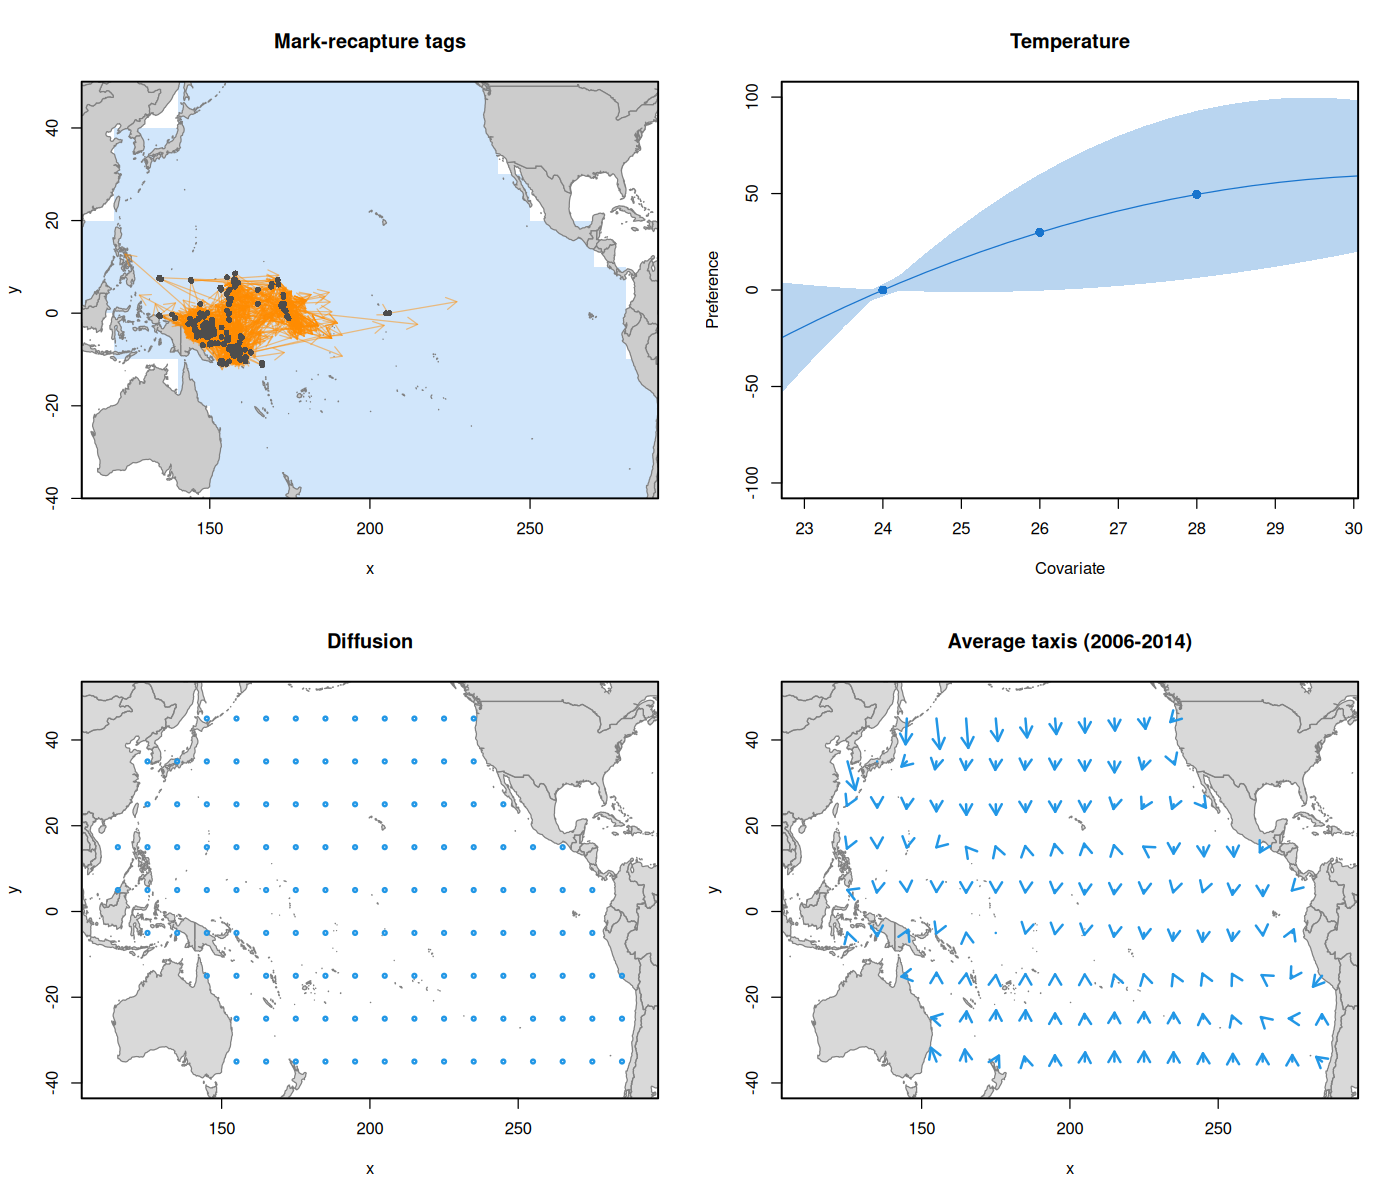
\includegraphics[width=\textwidth]{dtu_prototype}
  \caption{Snapshot of the DTU spatio-temporal model analyzing a small subset of
    the WCPO skipjack tagging data.\label{fig:dtu-prototype}}
\end{figure}

\vspace{2ex}

\textit{Enhancing and extending the DTU spatio-temporal model}

For the purposes of tuna assessments, the DTU spatio-temporal model currently
serves as a useful tool for analyzing tagging data externally from the
assessment model to produce abundance indices, which can faciliate transitioning
tuna assessments from MULTIFAN-CL to other software. The spatio-temporal model
also estimates movement coefficients, which can be used in a stock assessment
model.

When the earlier results from the IATTC-DTU analysis of EPO skipjack tagging
data were presented and reviewed at the SPC-DTU 2025 workshop in Copenhagen, it
was identified that improvements can still be made in the methodology. Areas
that could be enhanced involve the use of effort data and the application of the
Lincoln-Petersen mark-recapture estimator. During the initial exploration of
fitting the spatio-temporal model to WCPO skipjack tags, it was also apparent
that further development would be required to run the analysis using parallel
computing, given the very large WCPO skipjack tagging dataset. Tagging data are
known to be particularly influential in the WCPO skipjack assessment, which
makes it important to ensure that the best available statistical methods are
used to produce the resulting abundance indices.

Another development direction worth exploring is that the DTU spatio-temporal
model could conceivably be extended considerably in the future, to become a full
stock assessment model. This design concept was outlined by the DTU team at the
2025 workshop in Copenhagen. As a spatio-temporal model operating at a fine
spatial scale, it currently keeps track of key quantities such as natural and
fishing mortalities at each location. Thus, it already contains many elements of
a stock assessment model, if processes such as recruitment and fitting to length
composition data could be added. It is worth noting that the wider DTU team is
responsible for designing and implementing the latest generation of models used
in current European stock assessments, such as SAM and SPiCT. This means that
their current speculations about extending the spatio-temporal model to become a
full assessment model should be taken seriously and might become highly relevant
for future tuna assessments. Unlike existing stock assessments, this would be a
statistical framework that incorporates movement, environmental variables, and
other processes at a fine scale, rather than the somewhat arbitrary and very
large rectangular regions used in today's tuna assessments.

A preliminary outcome of the current scoping project is to recommend funding the
DTU team to enhance features and explore extensions of the spatio-temporal
model, as described above. WCPFC funding of DTU research efforts into this new
domain in fisheries science would make it more likely that operational stock
assessment software would be successfully developed. Secondly, funding and
collaboration would make it more likely that the resulting software would have
the design focus and features that directly address the requirements of WCPFC
tuna assessments.

As of mid 2025, it is too early to lay out a precise work plan for enhancing and
extending of the spatio-temporal model. However, the latest development version
of the R package is now close to having all the basic features of the model in
place, which will complete the core foundation before work can start to further
enhance and explore extensions of the model. The SC21 meeting is an opportune
time to discuss the possible prioritization and funding of this work stream that
can be formalized in 2026, a software development project focusing on enhancing
and extending the spatio-temporal model. For this reason, we suggest that a
small informal working group could be convened by the SC to discuss the
potential scope, deliverables, timeline, and resources for this and compare the
three development work streams that have the potential to develop
next-generation stock assessment software to be used in future tuna assessments.

The development work on enhancing and extending the spatio-temporal model would
be carried out by the team of statisticians at the Technical University of
Denmark, based in Copenhagen.

\vspace{2ex}

\subsubsection{FIMS tuna-specific modules}
\label{sec:fims-development-project}

\textit{Background}

The FIMS project aims to provide a modular and flexible design paradigm,
allowing scientists to choose and link together code modules to produce a stock
assessment model that is tailored for a particular assessment. The project has
currently developed a core module that allows the construction and fitting of
simple age-structured models. Early FIMS exploratory case studies have focused
on fitting to catch-at-age data, and the project is likely to initially
prioritize the needs of NOAA stock assessments in U.S. waters.

For the purposes of tuna assessments, it might be possible to design and develop
specific code modules to link with the FIMS core modules. Such tuna modules
could potentially provide a variety of features, adding basic model extensions
and/or introducing fundamental changes in the model structure.

\vspace{2ex}

\textit{Development of tuna-specific FIMS modules}

Before starting work on the potential design and development of full-featured
code modules, the first step will be to explore the technical procedures and
programming interface involved in producing FIMS-compatible modules. This
initial exploration should focus on very simple additions or model modifications
as a demonstration. After the technical exploration of such prototype FIMS
modules, the advantages and disadvantages of tuna-specific FIMS modules can be
evaluated against other forms of tuna stock assessment software development. See
the proposed SPC-FIMS workshop (\autoref{sec:fims-workshop}).

A preliminary outcome of the current scoping project is to recommend the
development of tuna-specific code modules that can be linked with core FIMS
modules to produce a model that is tailored for tuna stock assessment. Possible
examples of tuna-specific FIMS modules might provide some of the following
features:

\begin{itemize}
  \item Reference points specific for a tuna RFMO\\[-4.5ex]
  \item Improved handling of tagging data\\[-4.5ex]
  \item Explicit regions with fish movement coefficients\\[-4.5ex]
  \item Explicit age-length structured population array, rather than age only
\end{itemize}

As of mid 2025, it is too early to lay out a precise work plan for the
development of tuna-specific FIMS modules. However, recent milestones reached by
the FIMS project show that their software is now ready for a workshop focusing
on the technical procedures and programming interface involved in producing
FIMS-compatible modules. The SC21 meeting is an opportune time to discuss the
possible prioritization and funding of this work stream, a software development
project producing tuna-specific FIMS modules. For this reason, we suggest that a
small informal working group could be convened by the SC to discuss the
potential scope, deliverables, timeline, and resources for this and compare the
three development work streams that have the potential to develop
next-generation stock assessment software to be used in future tuna assessments.

The development work on tuna-specific FIMS modules could be carried out by a
consultant, working at SPC headquarters or remotely.

\vspace{2ex}

\subsubsection{IATTC designed tuna model}
\label{sec:iattc-tuna-model}

P123 has regularly reached out to experts in tuna stock assessments to discuss
development options for future tuna stock assessment software. In a recent
discussion, Mark Maunder (IATTC) shared his perspective that there is a need for
a new general model that can be applied in tuna stock assessments. In his words,
there are structural design issues to be considered, such as:

\begin{itemize}
  \item Spatial structure (e.g., fine scale spatio-temporal models)\\[-4.5ex]
  \item Length based dynamics\\[-4.5ex]
  \item Random effects\\[-4.5ex]
  \item Tagging data\\[-4.5ex]
  \item Close kin mark-recapture\\[-4.5ex]
  \item Multi-species
\end{itemize}

\vspace{2ex}

In his view, if he was asked to design a new model for tuna assessments today,
this is what he would probably do:

\begin{itemize}
  \item Large block spatial structure\\[-4.5ex]
  \item No length based dynamics\\[-4.5ex]
  \item Include random effects\\[-4.5ex]
  \item No tagging data\\[-4.5ex]
  \item Hopefully close kin mark-recapture can be added later easily\\[-4.5ex]
  \item No multi-species
\end{itemize}

\vspace{2ex}

This outline of a model design seems like an achievable model to implement, with
a high probability of success. For the purposes of this scoping project, an
initial evaluation of this model highlights the following key benefits:

\begin{itemize}
  \item New codebase in RTMB that will be relatively small, easy to modify and
  extend\\[-4.5ex]
  \item Keeping it simple, just focusing on the priority needs of tuna
  assessments\\[-4.5ex]
  \item Random effects, useful for allowing processes to vary in time and
  possibly between regions
\end{itemize}

\vspace{2ex}

The design reflects the new paradigm adopted by IATTC to analyze tags using
spatio-temporal analysis outside the assessment model, and for WCPFC maybe
contingent on acceptable performance of that approach. Given the growing
importance of the ability to incorporate CKMR data in tuna assessments, a
development project would take into account that this important model capability
would be added as the next milestone after achieving the core functionality
listed above. It is worth noting that the SBT stock assessment model that
incorporates CKMR data started off as a model without this feature, which was
added later (Rich Hillary, pers. comm.).

Mark Maunder has proposed organizing an online CAPAM workshop
(\autoref{sec:capam-online-workshop}) with tuna RFMOs and invited experts to
discuss the structural components of this tuna model design.

As of mid 2025, it is too early to lay out a precise work plan for developing
the IATTC designed tuna model. However, with the current plan of organizing an
online CAPAM workshop on this topic, it is likely that the model design stage
may progress fast in the coming months and initial development could start after
that. The SC21 meeting is an opportune time to discuss the possible
prioritization and funding of this work stream that can be formalized in 2026, a
software development project focusing on the IATTC designed tuna model. For this
reason, we suggest that a small informal working group could be convened by the
SC to discuss the potential scope, deliverables, timeline, and resources for
this and compare the three development work streams that have the potential to
develop next-generation stock assessment software to be used in future tuna
assessments.

\vspace{3ex}

\subsubsection{Adaptive plan}

\textit{Uncertainty and risks}

It is important to acknowledge the inherent uncertainty around the evolution of
next-generation stock assessment software. A general conclusion from reaching
out to the scientific community is the consensus that one cannot reliably
predict which of the current research and development directions will be most
relevant and useful for future tuna assessments.

The proposed development work streams outlined above are subject to considerable
uncertainty and risks:\\[-3ex]

\begin{itemize}
  \item The DTU spatio-temporal full assessment model design might involve
  complexities and levels of detail that are beyond the available information in
  tuna assessments, where data are often sparse and subject to imperfect
  sampling. Even if successfully developed, such a model might not be estimable
  or practical as a basis for providing management advice.\\[-2.5ex]
  \item The FIMS project might develop an overly complex framework architecture
  that results in slower progress and lower levels of code contributions than
  anticipated. A possible outcome could be that FIMS software cannot be used in
  future tuna assessments.\\[-2.5ex]
  \item The IATTC designed model resembles currently used models and has a lower
  level of uncertainty and risk than the other development options. It seems
  likely that this model could be used in future tuna assessments, although
  certain WCPFC-specific features may be needed.
\end{itemize}

\newpage

The recommended strategy to succeed in the face of uncertainty is to be active
and adaptive. Being active means investing resources into collaborative research
and development of new stock assessment methods and software. This will improve
the general outcomes in terms of the quality of the science. Being adaptive
means incorporating new scientific information and findings as they emerge and
alter the direction accordingly.

Another part of a successful strategy towards transitioning the WCPFC stock
assessments from MULTIFAN-CL will be to strengthen the partnerships with DTU and
IATTC.

\vspace{2ex}

\subsubsection{Partnerships}

\textit{DTU as a key provider of model development}

The scientific community regards the team of statisticians at the Technical
University of Denmark (DTU) as a preeminent research group developing
next-generation stock assessment methods and software. The programming
environments TMB and RTMB, the state-space stock assessment models SAM and
SPiCT, and the spatio-temporal model described above are only some of the
examples where the DTU team has introduced new paradigms for how fisheries
science is conducted.

The DTU team benefits from internal access to each other within the workplace.
For example, during their initial development of their spatio-temporal model,
Tobias Mildenberger and Anders Nielsen realized that the design of TMB was
preventing them from using a certain computational approach. Discussing their
findings with Kasper Kristensen, he identified a way to significantly alter and
improve the overall design of TMB to support this type of computational
approach. Other members of the DTU team include Casper Berg, Christoffer
Albertsen, and Vanessa Trijoulet, with Anders Nielsen as the team coordinator.

\vspace{2ex}

\textit{IATTC as our closest collaborator}

The best outcome for SPC would be to use stock assessment software that is also
used outside of SPC. In practical terms, the software used by other tRFMOs will
be especially relevant for identifying the best software for the WCPFC tuna and
billfish stock assessments. Among the tRFMOs, IATTC has a particularly high
research and development capacity and a long history working closely with SPC
researching stocks whose distribution often straddles the management boundaries
between the WCPO and EPO. IATTC and SPC regularly collaborate in peer reviews
and workshops to share ideas, experiences, and new methods for tuna and billfish
assessments.

Given the benefits of using the same software as other tRFMOs, it seems sensible
to coordinate, consult, and collaborate with IATTC when the time seems right to
move a certain assessment from one software platform to another.

\vspace{2ex}

\hypertarget{link:tor-8}{}
\subsection{TOR work area 8 (2025)}
\label{sec:tor-8}

\begin{quote}\sf
  Communicate with tuna RFMOs and other research labs to establish which RFMOs
  and labs are willing and able to commit scientist time to collaborate on
  specific tasks of the scoping project, as well as the upcoming main project.
\end{quote}

\vspace{2ex}

A list of ten questions was circulated to all the tuna RFMOs, to inform the
scoping project about current and future tuna stock assessment software.

\begin{enumerate}
  \item What assessment software do you use for tuna and billfish assessments?
  If possible, can you indicate which software is used for which stock?
  \item Are these software adequate for your current needs?
  \item Do you the think they will still be adequate in 10 years? If not, what
  are the likely main inadequacies?
  \item How important is explicit regional structure for the assessment and
  management of tuna and billfish stocks for your RFMO?
  \item Are tagging data important for any of your assessments? If so, which
  assessments?
  \item Given that Stock Synthesis is entering a sunset phase, do you have a
  strategy or plans in place for a post Stock Synthesis era? If yes, can you
  provide a brief description of your strategy or plans?
  \item How closely do you follow ongoing FIMS developments? Are you directly
  involved in discussions or experimental development?
  \item Do you have any ongoing development work on improving existing stock
  assessment software or developing new software? If yes, can you provide a
  brief description?
  \item Would you be willing to work collaboratively on the evaluation and/or
  development of software tailored for tuna assessments? If yes, is it likely
  that resources or scientist time might be available for this?
  \item Would your team be interested in attending an online CAPAM workshop
  focusing on current and future development of new stock assessment platforms
  to meet the needs of future tuna assessments?
\end{enumerate}

\vspace{2ex}

The responses from the tuna RFMOs are available on the project
\href{\tree/notes/rfmo_discussion/feedback}{website}.

In the response to question 9, regarding the ability to commit scientist time to
collaborate in the development and testing of stock assessment software, the
tuna RFMOs generally indicate a positive interest and emphasize the importance
of collaboration between the tuna RFMOs.

\vspace{2ex}

\hypertarget{link:tor-9}{}
\subsection{TOR work area 9 (2025)}
\label{sec:tor-9}

\begin{quote}\sf
  Communicate with tuna RFMOs and the FIMS project team to evaluate whether
  joint software development by tuna RFMOs could produce FIMS code modules, with
  the aim to develop future tuna assessment models using FIMS modules.
\end{quote}

\vspace{2ex}

In the response to question 7 in the above questionnaire, and more specifically
in follow-up discussions, the tuna RFMOs indicate different views on the FIMS
project. IOTC indicated that they had not been following the FIMS project, while
IATTC and CCSBT have expressed reservations about the potential of FIMS to
produce software relevant for future tuna assessments. Their recommendation is
to develop new tuna assessment software in RTMB that could be used by the tuna
RFMOs, rather than investing resources in producing FIMS-compatible modules.

The scoping project remains slightly more optimistic about the potential of FIMS
to produce software relevant for future tuna and billfish assessments. After
reaching out to the FIMS project, the conclusion from the discussion is to plan
a joint workshop to explore the development of tuna-specific FIMS modules. See
the proposed SPC-FIMS workshop (\autoref{sec:fims-workshop}).

\vspace{2ex}

\section{Other recent project activitites}

\subsection{SPC-DTU workshop to analyze tagging data}
\label{sec:dtu-2025-workshop}

\textit{DTU workshop background}

One challenge with transitioning tuna assessments from MFCL is that it is
considered the best statistical implementation of incorporating tagging data in
an integrated assessment model. Other software tend to use slightly less
sophisticated methods for incorporating tags. When discussing this challenge
with Mark Maunder (IATTC), he pointed out that in the 2024 EPO skipjack
assessment, IATTC had good success analyzing the tagging data externally, rather
than inside the stock assessment model. In this approach, a spatio-temporal
model is used to analyze the tagging data to produce abundance indices, which
are a basic input data type that can then be incorporated into any stock
assessment model.

This spatio-temporal model (Mildenberger et al. 2024) is a recent innovative
model that was developed by Tobias Mildenberger and Anders Nielsen at DTU in
collaboration with Mark Maunder. After a round of discussion among the members
of the scoping project, it was decided to fast-track and organize a technical
workshop to explore the feasibility of using this modeling approach to analyze
WCPO skipjack tagging data.

The workshop was held at DTU in Copenhagen 12--16 May 2025. Participants were
Arni Magnusson, Joe Scutt Phillips, and Inna Senina from SPC, and Anders Nielsen
and Tobias Mildenberger from DTU. Part-time attendees were Mark Maunder and
Rujia Bi from IATTC (short online meeting) and Colin Millar from ICES. John
Hampton contributed to workshop discussions via email during the week. The
scoping project used the opportunity to reach out to the wider team of
statisticians at DTU, discussing RTMB model development with Kasper Kristensen,
Casper Berg, Vanessa Trijoulet, and Molly Brooks.

\vspace{2ex}

\textit{DTU workshop activities}

With SPC and DTU presentations and discussions, we laid the foundation of a
collaborative project to analyze the WCPO tagging data using the DTU
spatio-temporal model.

During the workshop, Tobias Mildenberger developed an early prototype demo
model, using a small subset of the WCPO tagging data. The model estimates a
number of parameters describing the effect of environmental variables on
movement, in the form of preference functions using splines
(\autoref{fig:dtu-prototype}). The prototype model developed during the workshop
does not produce biomass indices, which is a subsequent step in the analysis.
The preliminary analysis conducted during the workshop confirmed that the data
are in the right format, ready for the upcoming analysis.

An observation made during the workshop is the overall similarity or
commonalities between SEAPODYM and the DTU spatio-temporal model. Some of the
relevant differences include the design objectives and research focus of these
models, the team composition behind the two models, and the availability of the
team to conduct a study that aims to produce abundance indices and other stock
assessment uses.

The workshop presentations, notes, and report are available on the scoping
project \href{\tree/workshops/2025-05-copenhagen}{website}, along with
analytical scripts and results.

\vspace{2ex}

\textit{DTU workshop follow-up}

See the proposed follow-up project activity to support enhancing and extending
the spatio-temporal model (\autoref{sec:dtu-support-tagging}).

\vspace{2ex}
\newpage

\section{Recommendation of project activities in 2025--2026}

Areas for discussion and prioritization in the small IWG at SC21 include:

\vspace{0.5ex}

\subsection{Collaborate with IATTC and others on the design of a new tuna model}
\label{sec:capam-online-workshop}

Mark Maunder has proposed organizing an online CAPAM workshop with tuna RFMOs
and invited experts to discuss the structural components of a possible future
tuna assessment model design (\autoref{sec:iattc-tuna-model}).

It would be beneficial for the scoping project to have an active support role in
organizing and conducting the workshop. The timing of this workshop is to be
decided. The workshop outcomes and follow-up model design work may lead to the
development of future tuna assessment software that can be used by many tuna
RFMOs.

\vspace{2ex}

\subsection{Tuna RFMO workshop to review Stock Synthesis modeling techniques}
\label{sec:ss-modeling-techniques}

Transitioning the two WCPFC billfish assessments to Stock Synthesis has been a
learning process that required new knowledge, tools, and technical solutions.
The increased interaction with the wider scientific community has already proved
to be an important benefit from using a widely used software platform for these
assessments (\autoref{sec:tor-5}). See also the overview and evaluation of Stock
Synthesis (\autoref{sec:ss-software-evaluation}).

It would be beneficial for the billfish assessments and possibly future tuna
assessments to bring together scientists who have experience and expertise in
configuring and diagnosing tuna and billfish assessments in Stock Synthesis.

The WCPFC assessments of swordfish and striped marlin in 2025 highlighted that
there are aspects of SS3 that need to be better understood about the calculation
of fishing mortality and reference points. In addition to resolving those
important issues, the workshop could also focus on the model settings and
results from the EPO 2024 skipjack assessment, which used SS3 with abundance
indices from the external DTU spatio-temporal model. The WCPO skipjack
assessment will transition from MULTIFAN-CL at some point, and Stock Synthesis
with external tagging analysis is one option to be considered for the 2028
assessment.

SPC could organize such a workshop jointly with other tuna RFMOs. The timing of
this workshop is to be decided.

\vspace{2ex}

\subsection{Support DTU analysis of WCPO skipjack tagging data}
\label{sec:dtu-support-tagging}

The next step in the DTU analysis of WCPO skipjack tagging data is to secure
funding for the DTU team to work on the spatio-temporal model development and
analysis. The timeline of the project will be aligned with the 2028 WCPFC
skipjack assessment, so the final model results should be delivered by the end
of 2027. Intermediate milestones will be planned after funding has been secured,
possibly organizing a second workshop to discuss and decide on model options.

See the SPC-DTU 2025 workshop (\autoref{sec:dtu-2025-workshop}) for the work
completed so far, as well as further details about the analysis, along with
possible enhancements and extensions of the DTU spatio-temporal model
(\autoref{sec:dtu-development-project}).

\vspace{2ex}

\subsection{Explore the possibility of using the SBT model code}
\label{sec:sbt-model-code}

The scoping project has reached out to the team of scientists involved in the
SBT assessment and will discuss further the possibility of using their model
code as a starting point for developing new software for the South Pacific
albacore assessment, incorporating CKMR data. IATTC is also involved in this
discussion, as albacore is a joint assessment between WCPFC and IATTC.

See the overview and evaluation of the SBT stock assessment software
(\autoref{sbt-software-evaluation}).

\vspace{2ex}

\subsection{Develop Gadget model for single-area yellowfin dataset}
\label{sec:yft-gadget}

The scoping project has reached out to the Gadget development team (Bjarki
Elvarsson and Jamie Lentin) to explore the possibility of fitting a Gadget model
to the single-area yellowfin dataset that was prepared as part of the scoping
project (\autoref{sec:tor-6}).

It would be beneficial for the scoping project to gain first-hand experience
fitting a Gadget model to a large tuna dataset that consists of 280 quarterly
time steps, 40 quarterly ages, 95 length bins, and 32 fisheries. This can help
the scoping project gain insights from using an explicitly age-length structured
model to analyze tuna data and get a rough estimate of the computational
overhead of age-length models. Gadget represents certain state-of-the-art
statistical methods of interest, and examining the model configuration, results,
and diagnostics will be a useful reference for designing any future tuna
assessment software. See the overview and evaluation of Gadget
(\autoref{sec:gadget-software-evaluation}).

\vspace{2ex}

\subsection{SPC-FIMS workshop to explore linking FIMS modules}
\label{sec:fims-workshop}

The scoping project has identified the usefulness of exploring the technical
procedures and programming interface involved in producing FIMS-compatible
modules. This initial exploration should focus on very simple additions or model
modifications as a demonstration. After the technical exploration of such
prototype FIMS modules, the advantages and disadvantages of tuna-specific FIMS
modules can be evaluated against other forms of tuna stock assessment software
development.

See the overview and evaluation of the FIMS project
(\autoref{sec:fims-software-evaluation}), as well as the possible development
work stream (\autoref{sec:fims-development-project}). The timing of this
workshop is to be decided.

\vspace{2ex}

\subsection{Formal proposal for WCPFC software development project}
\label{sec:development-proposal-sc22}

This year's progress report outlines a potential development project, describing
possible development work streams that are currently being evaluated (see
\autoref{sec:tor-7}).

The scoping and evaluation will continue for the work period from August 2025 to
August 2026, with a formal development project proposal to be presented at SC22
as a key outcome from the scoping project.

\vspace{4ex}

\section{References}

\sloppy\setlength\hyphenpenalty{1000}

\begin{description}\setlength\itemsep{0ex}
  \item Bi, R., M.N. Maunder, H. Xu, C. Minte-Vera, J. Valero, and A.
  Aires-da-Silva. 2024. Stock assessment of skipjack tuna in the eastern Pacific
  Ocean: 2024 benchmark assessment. IATTC Document SAC-15-04. 59 pp.
  \href{https://www.iattc.org/GetAttachment/f57dece1-81ba-4771-8fa8-3362320a368%
    a/SAC-15-04_Skipjack-tuna-benchmark-assessment-2024.pdf}{Available online}
  \item Fournier, D.A., J. Hampton, and J.R. Sibert. 1998. MULTIFAN-CL: A
  length-based, age-structured model for fisheries stock assessment, with
  application to South Pacific albacore, \textit{Thunnus alalunga}. Can. J.
  Fish. Aquat. Sci. 55:2105--2116.
  \item Magnusson, A. and M. Maunder. 2025. fishgrowth: Fit growth curves to
  fish data. R package version 1.0.2.
  \href{https://doi.org/10.32614/CRAN.package.fishgrowth}
  {doi: 10.32614/CRAN.package.fishgrowth}
  \item Magnusson, A. and N. Davies. 2024b. Scoping the next stock assessment
  platform, stage I:\linebreak Reaching out to tuna RFMOs and the scientific
  community. Presented at the SPC international expert meeting, 13 May and 18
  June 2024. 31 pp.
  \href{\present/2024_05_13_experts_scoping/2024_05_13_experts_scoping.pdf}
  {Available online}
  \item Mildenberger, T.K., A. Nielsen, and M. Maunder. 2024. A spatiotemporal
  Petersen-type model for skipjack in the EPO. IATTC Document SAC-15 INF-G. 19
  pp. \href{https://www.iattc.org/GetAttachment/f8eacbc8-92b8-434d-a331-bdc733d%
    c1bc6/SAC-15-INF-G_Spatiotemporal-tagging-model-for-skipjack-in-the-EPO.pdf}
  {Available online}
  \item Mildenberger T., M. Maunder, and A. Nielsen. 2025. momo: Tagging-based
  movement modeling. R package version 0.0.0.9000.
  \href{https://github.com/tokami/momo}{https://github.com/tokami/momo}
  \item Punt, A.E., A. Dunn, B.Þ. Elvarsson, J. Hampton, S.D. Hoyle, M.N.
  Maunder, R.D. Methot, and A. Nielsen. 2020. Essential features of the
  next-generation integrated fisheries stock assessment package: A perspective.
  Fish. Res. 229:105617.
\end{description}

\newpage

\appendix

\section{Appendix: Single-region YFT2023 model}
\label{sec:yft-mfcl}

\vspace{1ex}

Nick Davies\\
1 July 2025

\vspace{1ex}

\subsection*{Summary}

As part of the P123 project ``Scoping the next Stock Assessment software'', a
step includes the preparation of a simplified tuna stock assessment model and
input data set. This report presents the preliminary results of this step using
the yellowfin tuna stock assessment model as was developed in 2023. The original
model was spatially stratified into 5 defined regions. A simplified version was
developed using MULTIFAN-CL having no spatial stratification (a single region),
while retaining the original fisheries definitions for the 32 capture fisheries,
and their fishery-specific input data structures. Instead of the five
region-specific survey fisheries for which CPUE indices were available, the
simplified model defined a single survey fishery representative of the entire
model domain. The simplified model was fitted and achieved convergence, and a
comparison with the original multi-region model is presented here.

\vspace{1ex}

\subsection*{Method}

The existing YFT2023 diagnostic case model that employs the catch-conditioned
method was used for preparing the input data, and to demonstrate the application
of MULTIFAN-CL to a spatially unstratified tuna data set.

\vspace{1ex}

\textit{De-stratification of the model spatial configuration and observations}

The input files that specify the spatial stratification, recruitment and
movement parameterisations (*.ini and *.frq) were duly modified to define a
single region with no movement diffusion coefficients or spatial recruitments.
All fisheries and all tagging release events were defined to occur in the same
single region. All other fishery-specific observations (size compositions,
catch, effort, conditional age-length data) for the capture fisheries (1 to 32)
were retained without modification; as these fisheries were re-defined as
occurring in the single region. A single standardized CPUE time series was
available for the survey fisheries combined over all 5 regions, and was taken as
being representative of the entire model domain, i.e., a single-region index.
Similarly, the size composition data among all five survey fisheries were
aggregated into a single data set. This single survey fishery (33) was defined
as such for the simplified model. Estimates of temporal precision for the CPUE
indices were available, allowing a concentrated CPUE likelihood to be estimated
for the simplified model.

The initial MULTIFAN-CL -makepar operation was completed, and the
resultant 00.par file structure was assessed for correctly excluding all spatial
stratification or movement parameterisation. All phases of the doitall
minimization that originally included spatial parameter estimation, were
modified to de-activate the estimation of these parameters. The phase 1
operation was successfully completed, and then all subsequent phases of the
minimization run to convergence.

The models included in this comparison were:

\begin{small}
  \begin{tabular}{ll}
    mult\_regs             & - original YFT2023 diagnostic case model, having
                             multiple (5) regional strata\\[1ex]
    sngl\_reg\_cpue1       & - simplified single-region model, employs
                             non-concentrated CPUE likelihood\\[1ex]
    sngl\_reg\_conc\_cpue1 & - simplified single-region model, employs
                             concentrated CPUE likelihood\\[1ex]
  \end{tabular}
\end{small}

\vspace{1ex}

\subsection*{Results}

Both the single-region models produced stable minimisations with converged
solutions obtained (maximum gradients $\sim$2.0e-04). Whereas the
multi-region model produced a positive definite Hessian (PDH) solution, neither
of the single-region models were PDH solutions (Table 1).

In respect of the size-composition data, comparable fits to the
length-frequencies were obtained among the models, but markedly worse
weight-frequency fits were obtained for the single-region models (21\% worse
negative-log likelihood) (Table 1). Similarly, worse fits were obtained to the
tagging data (9.6\% worse negative-log likelihood). Slightly better (1.1\%) fits
were obtained to the conditional age-length data by the single-region models.
There was negligible difference in the fit to the CPUE indices among the
single-region models (Figure 8), with that using the concentrated likelihood
differing only slightly in respect of the indices in the early time periods for
which temporal precision was low.

There were notable differences in the recruitment and natural mortality
estimates of the single-region models compared to the multi-region model.
Absolute recruitments were approximately 50\% lower in all time periods (Figure
2), but with similar temporal variation. The Lorenzen natural mortality function
was lower overall by on average approximately 10\%, which accorded lower
mortality, particularly for age classes $<$ 12 quarters (Figure 5). In contrast,
the growth function was almost identical (Figure 4). A number of the estimated
selectivity-at-age functions were more dome-shaped, or with lower right-hand
limbs (Figure 6).

Despite these differences in model fit to the observations and estimated
parameters, overall absolute biomass was generally similar among the multi- and
single-region models (Figure 1), and showed similar temporal variation.
Noticeable differences were however evident in the recent periods (the past 15
years), with absolute total biomass of the single-region models being 23\% lower
(Table 1). Despite this similarity, the estimated depletion of adult biomass is
at a 35\% lower level compared to the multi-region model (Table 1 and Figure 7).
Equilibrium quantities also differed, with MSY being 9.5\% lower, and unfished
total biomass (B0) being 8.6\% higher (Table 1).

These differences in the model derived variables can be attributed to the
various parameter estimates that differ among the multi- and single-region
models. It seems surprising that a model having substantially lower productivity
(50\% of the recruitments), yet sustains the equivalent total removals and
produces a comparable absolute abundance, with only 10\% lower equilibrium
yield. Notably, the lower Lorenzen natural mortality over all age classes
substantially reduces the total mortality; hence, B0 is higher. The more
dome-shaped selectivities and being lower for older age classes, reduces fishing
mortality for the older age classes and allows for ``cryptic'' biomass, and
increases MSY. Also, the spatial dynamics of the multi-region model in respect
of recruitment, movement and fishing mortality on sub-populations may increase
the overall fishing mortality estimates. Whereas, the fishing mortality of all
fisheries acting upon a single population serves to exclude the effects of high
impacts on sub-populations.

The combined effects of the above parameter differences can accord higher
resilience of the single-region model to fishing mortality. However, the lower
natural mortality rate contributes to greater estimated depletion, indicating
the relative fishing impact is higher. A closer examination of the estimated
adult depletion within the equatorial regions of the multi-region model (regions
2, 3 and 4) reveals substantial regional differences, with that of region 2
being very similar to the estimated level of the single-region models. This
might indicate a dominant effect of the region 2 observations upon the
single-region model estimates.

\newpage

\section*{Tables and Figures}

\begin{small}
  Table A.1. Comparison of selected model parameters, negative log-likelihood
  terms and derived quantities,\\[-1ex]
  for the multi-region (mult\_regs) and single-region models (sngl\_reg\_cpue1,
  sngl\_reg\_conc\_cpue1).
\end{small}

\begin{footnotesize}
  \begin{tabular}{lrrrrr}
    \hline
    Model quantity
    & mult\_regs
    & sngl\_reg\_cpue1
    & sngl\_reg\_conc\_cpue1
    & \%diff\_nonconc
    & \%diff\_conc\\
    \hline
    MSY & 169700 & 153500 & 153600 & -9.55 & -9.49\\
    Ccurr.MSY & 4.224 & 4.665 & 4.662 & 10.44 & 10.37\\
    Fmsy & 0.073 & 0.060 & 0.060 & -18.08 & -18.08\\
    Fmult & 1.676 & 1.209 & 1.206 & -27.86 & -28.04\\
    Fcurr.Fmsy & 0.597 & 0.827 & 0.829 & 38.63 & 38.97\\
    B0 & 8510000 & 9241000 & 9244000 & 8.59 & 8.63\\
    Bmsy & 2336000 & 2580000 & 2581000 & 10.45 & 10.49\\
    Bcurr & 4648625 & 3587013 & 3577813 & -22.84 & -23.04\\
    SB0 & 5347000 & 6573000 & 6576000 & 22.93 & 22.98\\
    SBmsy & 1072000 & 1440000 & 1440000 & 34.33 & 34.33\\
    SBcurr & 2404755 & 1996569 & 1991219 & -16.97 & -17.20\\
    Bcurr.Bmsy & 1.990 & 1.390 & 1.386 & -30.13 & -30.34\\
    SBcurr.SBmsy & 2.243 & 1.387 & 1.383 & -38.19 & -38.36\\
    SBcurr.SBcurrF0 & 0.454 & 0.296 & 0.295 & -34.92 & -35.08\\
    SBlatest.SBlatestF0 & 0.429 & 0.292 & 0.291 & -31.95 & -32.15\\
    obj\_bhsteep & 0.311 & 0.415 & 0.415 & 33.51 & 33.31\\
    obj\_lencomp & -154969.914 & -153345.580 & -153345.611 & -1.05 & -1.05\\
    obj\_wtcomp & -610342.171 & -483274.416 & -483273.668 & -20.82 & -20.82\\
    obj\_tagdata & 13217.201 & 14479.783 & 14479.435 & 9.55 & 9.55\\
    obj\_agelngdata & 2480.443 & 2452.738 & 2452.727 & -1.12 & -1.12\\
    obj\_cpue & -1157.645 & -314.031 & -313.991 & -72.87 & -72.88\\
    Obj & -750515.800 & -619859.458 & -619858.965 & -17.41 & -17.41\\
    No. parameters & 1901 & 445 & 445 & -76.59 & -76.59\\
    gradient & 0.0001268 & 0.0001774 & 0.0001527 & 39.90 & 20.46\\
    Lmin & 19.800 & 19.800 & 19.800 & 0.00 & 0.00\\
    Lmax & 141.958 & 141.924 & 141.923 & -0.02 & -0.02\\
    K & 0.132 & 0.132 & 0.132 & 0.03 & 0.03\\
    PDH & Yes & No & No & - & -\\
    \hline
  \end{tabular}
\end{footnotesize}

\newpage

\small

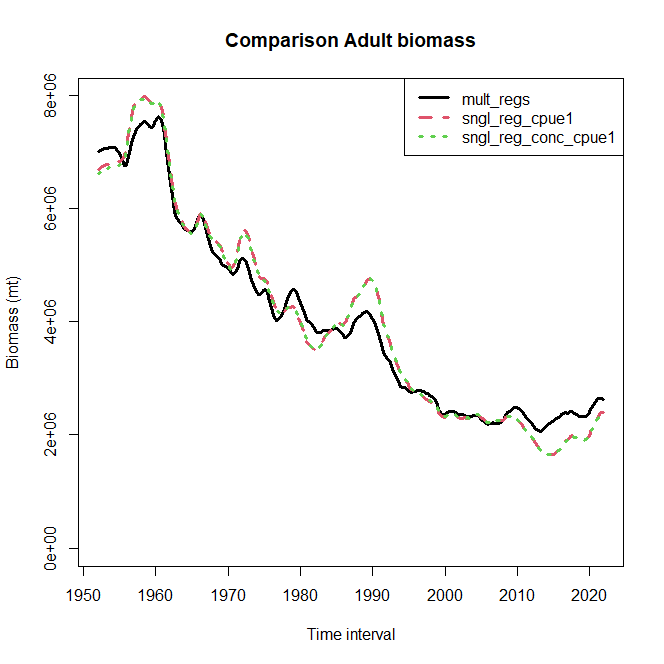
\includegraphics[width=0.58\textwidth]{yft_biomass}

Figure A.1. Comparison of adult biomass between the multi-region (mult\_regs)
and\\[-0.8ex]
single-region (sngl\_reg\_cpue1, sngl\_reg\_conc\_cpue1) models.

\vspace{1ex}

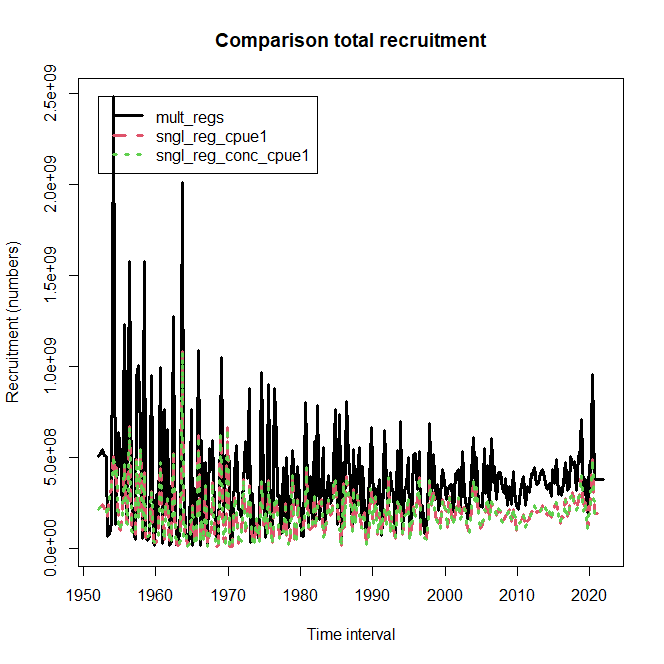
\includegraphics[width=0.58\textwidth]{yft_recruitment}

Figure A.2. Comparison of estimated absolute recruitment between the
multi-region (mult\_regs) and\\[-0.8ex]
single-region (sngl\_reg\_cpue1, sngl\_reg\_conc\_cpue1) models.

\vspace{1ex}

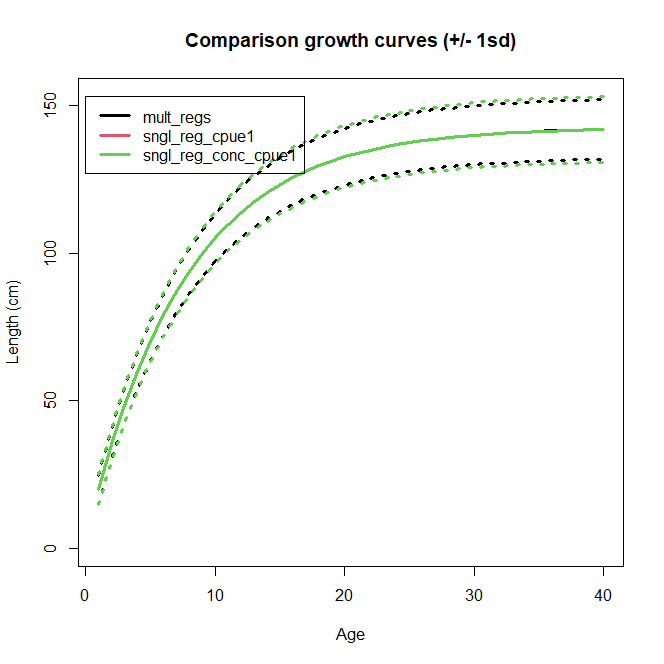
\includegraphics[width=0.58\textwidth]{yft_growth}

Figure A.4. Comparison of estimated von Bertalanffy growth between the
multi-region (mult\_regs) and\\[-0.8ex]
single-region (sngl\_reg\_cpue1, sngl\_reg\_conc\_cpue1) models.

\vspace{1ex}

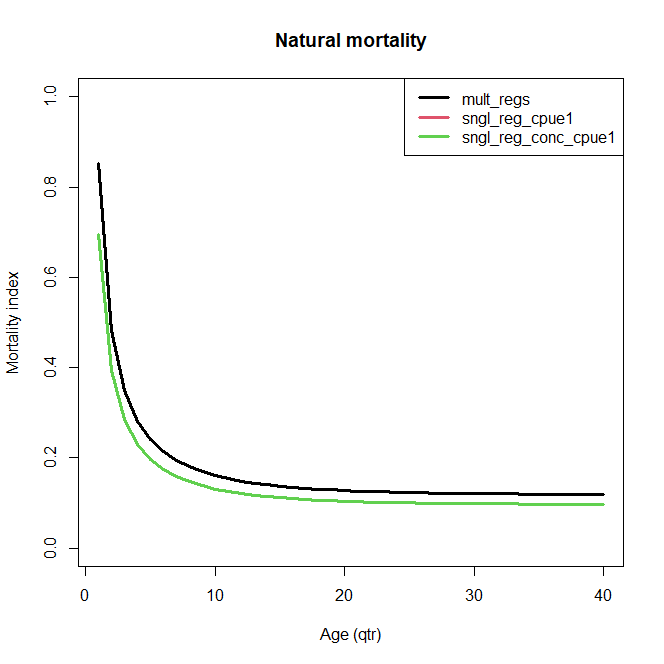
\includegraphics[width=0.58\textwidth]{yft_natmort}

Figure A.5. Comparison of estimated Lorenzen natural mortality functions between
the\\[-0.8ex]
multi-region (mult\_regs) and single-region (sngl\_reg\_cpue1,
sngl\_reg\_conc\_cpue1) models.

\vspace{1ex}

\newpage

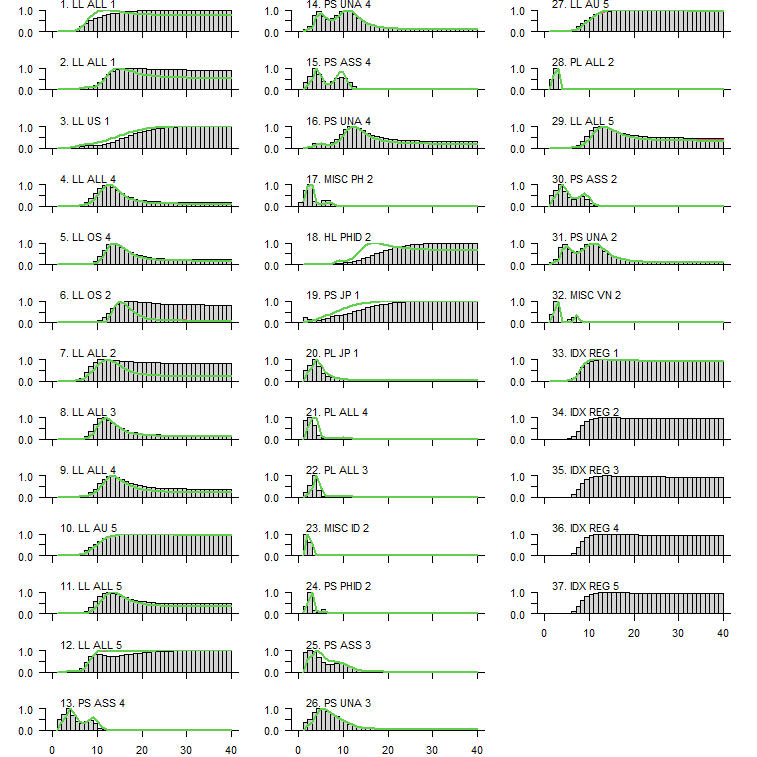
\includegraphics[width=\textwidth]{yft_selectivity}\\[1ex]

Figure A.6. Comparison of estimated selectivity-at-age between the multi-region
(mult\_regs, histograms)\\[-0.8ex]
and single-region (sngl\_reg\_cpue1, sngl\_reg\_conc\_cpue1, red and green
lines) models.

\vspace{1ex}

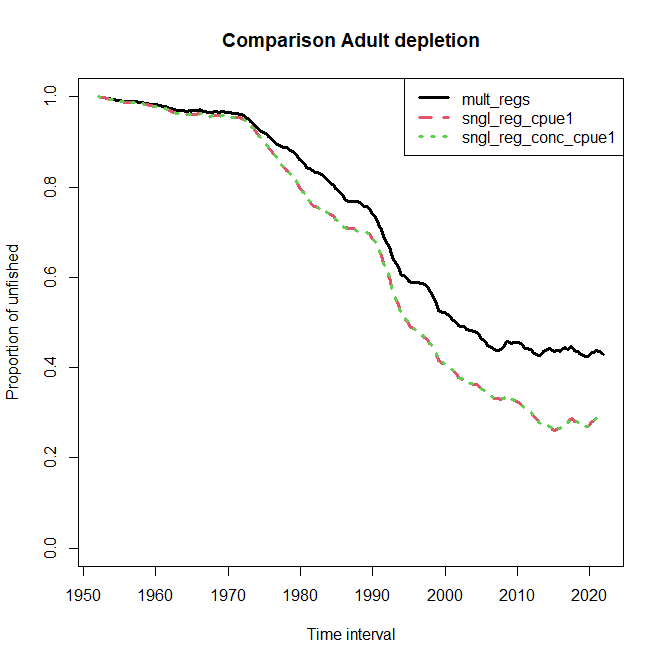
\includegraphics[width=0.58\textwidth]{yft_depletion_structure}

Figure A.7. Comparison of estimated spawning biomass depletion between the
multi-region (mult\_regs) and\\[-0.8ex]
single-region (sngl\_reg\_cpue1, sngl\_reg\_conc\_cpue1) models.

\vspace{1ex}

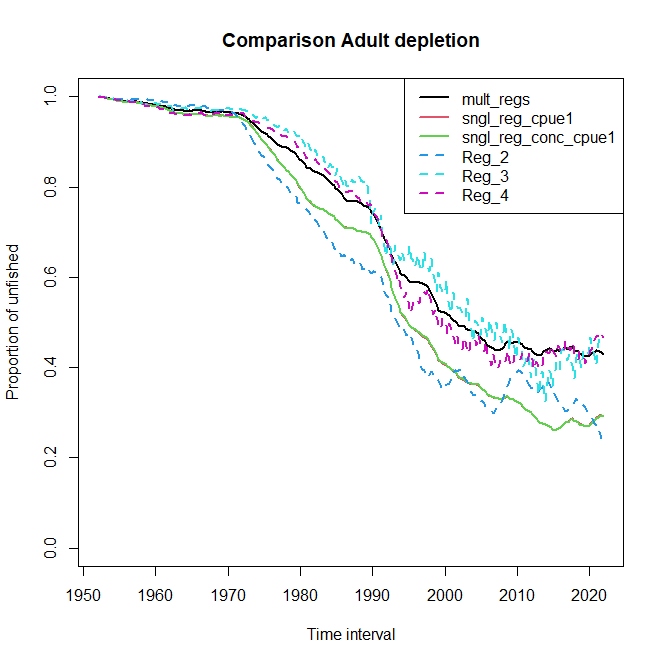
\includegraphics[width=0.58\textwidth]{yft_depletion_regions}

Figure A.8. Comparison of estimated spawning biomass depletion between\\[-0.8ex]
component regions of the multi-region model (Region 2, Region 3, Region
4)\\[-0.8ex]
and single-region (sngl\_reg\_cpue1, sngl\_reg\_conc\_cpue1) models.

\vspace{1ex}

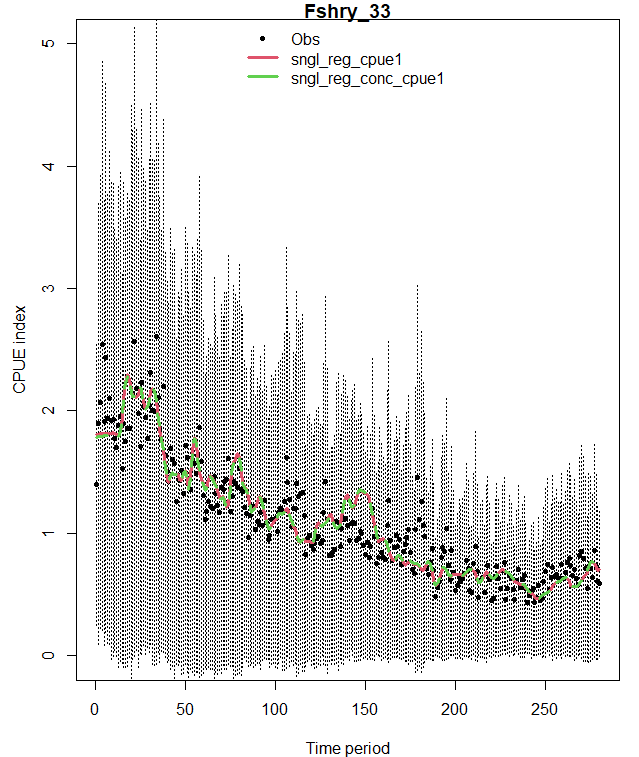
\includegraphics[width=11cm]{yft_cpue}\\[1ex]

Figure A.9. Comparison of the fit to the observed CPUE indices between the
single-region models employing\\[-0.8ex]
the non-concentrated (sngl\_reg\_cpue1), and
concentrated (sngl\_reg\_conc\_cpue1) likelihood formulations.\\[-0.8ex]
Vertical dashed lines are the index + or - CV.

\vspace{1ex}

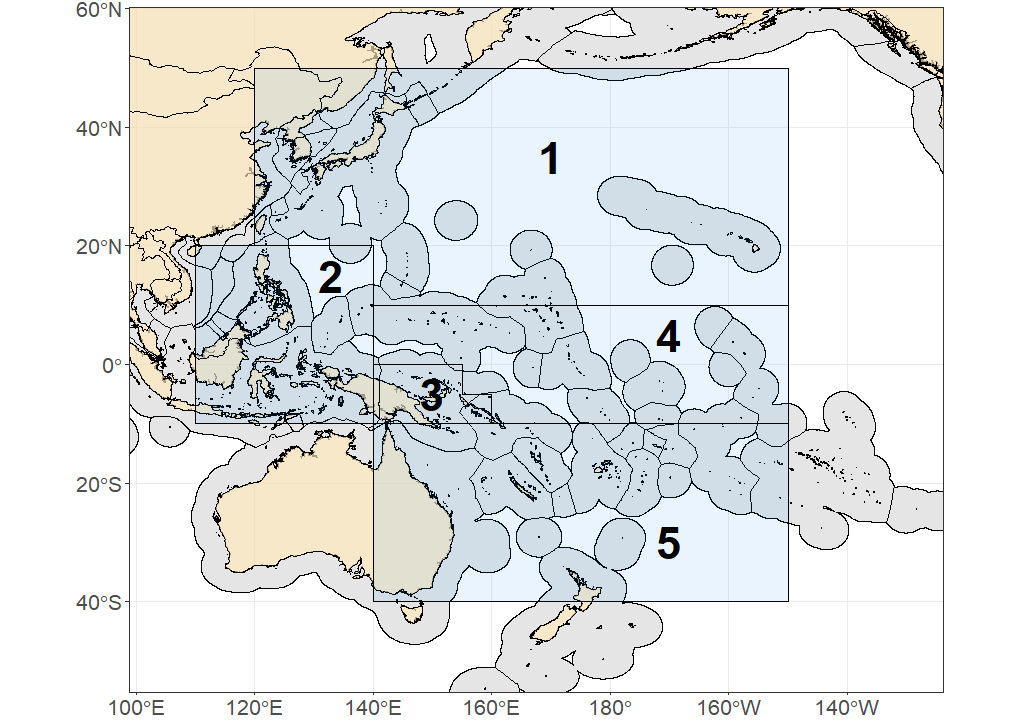
\includegraphics[width=11cm]{yft_map}\\[1ex]

The geographical area covered by the stock assessment and the
boundaries of the model regions\\[-0.8ex]
for the 5 region structure that was used for 2023 WCPO yellowfin tuna
assessment.

\end{document}
